\documentclass{article}
\usepackage[margin=0.75in]{geometry}
\usepackage{mymath}
\usepackage{subcaption}
\usepackage{tikz}

\title{Test Creator System Design}
\author{Nathan Gurrin-Smith}
\begin{document}
\maketitle

\section{Introduction}
This is a program that will be used to generate practice tests from a list of questions. It aims to help improve learning by encouraging frequent, interleaved testing.

\section{Use Cases}
\begin{itemize}
    \item Login,
    \item Add, view, edit, and delete presets,
    \item Add, view, edit, and delete questions,
    \item add, view, edit, and delete categories,
    \item generate practice tests
\end{itemize}

\newpage
\section{Technology}
The framework being used is PERN.

\subsection{Data}
\subsubsection*{Naming Conventions}
We will use the following naming conventions for our data model
\begin{itemize}
    \item Tables and columns will be in PascalCase.
    \item Tables and columns will be singular.
    \item Junction tables will be named JunctionTable1Table2
\end{itemize}
Note: PostgreSQL automatically forces lowercase internally, but we'll always reference by PascalCase.

Note: Because of the above note, we must reference all columns with lowercase in our javascript files.

\subsubsection*{Data Model}

We will have the following data model:

\begin{figure}[h!]
    \begin{subfigure}{\textwidth}
        \begin{tabular}{|c|c|c|}
            \hline
            \multicolumn{3}{|c|}{UserAccount} \\
            \hline
            UserAccountID & Username & Password \\
            \hline
        \end{tabular}
        \vspace*{2em}
    \end{subfigure}
    \begin{subfigure}{\textwidth}
        \begin{tabular}{|c|c|c|c|c|c|}
            \hline
            \multicolumn{6}{|c|}{Preset} \\
            \hline
            PresetID & Name & Preamble & Sep & Postamble & UserAccountID(FK) \\
            \hline
        \end{tabular}
        \vspace*{2em}
    \end{subfigure}
    \begin{subfigure}{0.2\textwidth}
        \begin{tabular}{|c|c|}
            \hline
            \multicolumn{2}{|c|}{Collection} \\
            \hline
            CollectionID & Name \\
            \hline
        \end{tabular}
        \vspace*{2em}
    \end{subfigure}
    \begin{subfigure}{0.4\textwidth}
        \begin{tabular}{|c|c|c|}
            \hline
            \multicolumn{3}{|c|}{SubCollection} \\
            \hline
            SubCollectionID & Name & CollectionID(FK) \\
            \hline
        \end{tabular}
        \vspace*{2em}
    \end{subfigure}
    \begin{subfigure}{0.3\textwidth}
        \begin{tabular}{|c|c|c|c|c|}
            \hline
            \multicolumn{4}{|c|}{Question} \\
            \hline
            QuestionID & Name & Content & Source \\
            \hline
        \end{tabular}
        \vspace*{2em}
    \end{subfigure}
    \begin{subfigure}{0.5\textwidth}
        \begin{tabular}{|c|c|}
            \hline
            \multicolumn{2}{|c|}{JunctionUserAccountCollection} \\
            \hline
            UserAccountID(FK) & CollectionID(FK) \\
            \hline
        \end{tabular}
        \vspace*{2em}
    \end{subfigure}
    \begin{subfigure}{0.5\textwidth}
        \begin{tabular}{|c|c|c|}
            \hline
            \multicolumn{3}{|c|}{JunctionUserAccountQuestion} \\
            \hline
            UserAccountID(FK) & QuestionID(FK) & LastReviewed \\
            \hline
        \end{tabular}
        \vspace*{2em}
    \end{subfigure}
    \begin{subfigure}{0.3\textwidth}
        \begin{tabular}{|c|c|}
            \hline
            \multicolumn{2}{|c|}{JunctionSubCollectionQuestion} \\
            \hline
            SubCollectionID(FK) & QuestionID(FK) \\
            \hline
        \end{tabular}
    \end{subfigure}
\end{figure}

Which are related via,
\begin{center}
    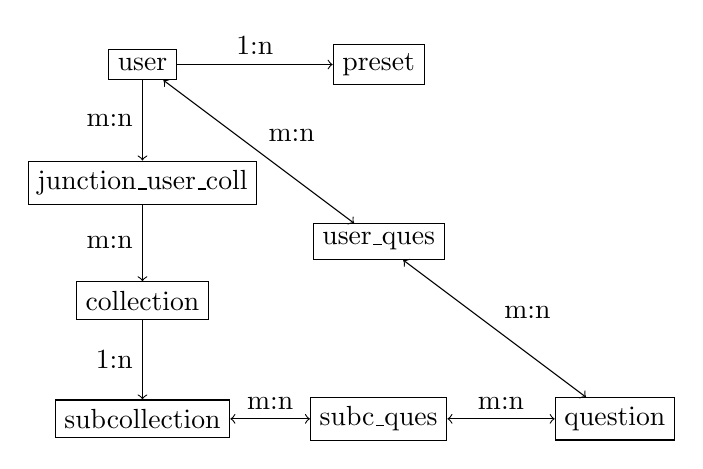
\begin{tikzpicture}
        \node[draw] at (0,0) (A) {user};
        \node[draw] at (3,0) (B) {preset};
        \node[draw] at (0,-1.5) (H) {junction\_user\_coll};
        \node[draw] at (0,-3) (C) {collection};
        \node[draw] at (0,-4.5) (D) {subcollection};
        \node[draw] at (3,-4.5) (E) {subc\_ques};
        \node[draw] at (6,-4.5) (F) {question};
        \node[draw] at (3,-2.25) (G) {user\_ques};

        \draw [->] (A) -- (B) node[midway,above] {1:n};
        \draw [->] (A) -- (H) node[midway,left] {m:n};
        \draw [->] (H) -- (C) node[midway,left] {m:n};
        \draw [->] (C) -- (D) node[midway,left] {1:n};
        \draw [<->] (D) -- (E) node[midway,above] {m:n};
        \draw [<->] (E) -- (F) node[midway,above] {m:n};
        \draw [<->] (A) -- (G) node[midway,above right] {m:n};
        \draw [<->] (G) -- (F) node[midway,above right] {m:n};
    \end{tikzpicture}
\end{center}

\textbf{Orphans:} Some of the properties above require a parent.
\begin{itemize}
    \item A Collection requires at least one parent UserAccount,
    \item A SubCollection requires a parent Collection,
    \item A Question requires a parent UserAccount and a parent SubCollection
    \item A Preset requires a parent UserAccount
\end{itemize}
Thus, when we delete a parent, we not only need to delete entries in the junction table, but also the entries in the child tables since, most frequently, the foreign keys will be stored in the junction table and not the child table. The ones that need this, that is, the ones that aren't handled by ON DELETE CASCADE, are orphaned collections and orphaned questions. So, we need to handle orphans when we delete:
\begin{itemize}
    \item Users (questions and collections)
    \item Subcollections (questions)
\end{itemize}


\subsection{Backend}
\subsubsection*{Routes}
We are using the \texttt{/api/} style.
\begin{itemize}
    \item All user related routes will be at /api/user/
    \item All preset related routes will be at /api/preset/
    \item All collection related routes will be at /api/collection/
    \item All subcollection related routes will be at /api/subcollection/
    \item All question related routes will be at /api/question/
\end{itemize}

\subsubsection*{Other Modules}
Here are the other modules we have,
\begin{itemize}
    \item dbClean.js: as mentioned above, we need to ensure orphaned entities are deleted, which this module handles.
\end{itemize}

\subsubsection*{Client}

\end{document}
